\documentclass{article}

\usepackage[dvips]{graphicx}
\usepackage{latexsym}
\usepackage{epsf}
\usepackage{epsfig}
\usepackage{color}
\usepackage{a4}
\usepackage{amssymb}
\usepackage{amsxtra}
\usepackage{fancyhdr}
\usepackage{enumitem}
\usepackage[margin=1in]{geometry}
\usepackage{amsfonts, amsmath, amssymb}
\usepackage[none]{hyphenat}
\usepackage{fancyhdr}
\usepackage{tabularx}
\usepackage{makecell}
\usepackage{float}
\usepackage{parskip}
\usepackage{multirow}
\usepackage{subcaption}
\usepackage{xcolor}
\usepackage{hyperref} %href
\usepackage[]{minted}
\usepackage{tcolorbox}
\usepackage{etoolbox}
\usepackage{amsmath}
\usepackage{xcolor}
\usepackage[ruled,vlined]{algorithm2e}
\newcommand\norm[1]{\left\lVert#1\right\rVert}
\SetKwRepeat{Do}{do}{while}
\BeforeBeginEnvironment{minted}{\begin{tcolorbox}}%
	\AfterEndEnvironment{minted}{\end{tcolorbox}}%

\definecolor{monokaibg}{HTML}{272822}
\definecolor{friendlybg}{HTML}{f0f0f0}
\definecolor{bg}{HTML}{282828} % from https://github.com/kevinsawicki/monokai


\definecolor{light-gray}{gray}{0.95} %the shade of grey that stack exchange uses
\usepackage{mdframed} %nice frames
\newenvironment{myenv}[1][]
{\begin{mdframed}[backgroundcolor=light-gray,linecolor = light-gray,font=\small,#1]\begin{tabbing}}
		{\end{tabbing}\end{mdframed}}
	
\newcommand{\HRule}[1]{\rule{\linewidth}{#1}}

\pagestyle{fancy}
\fancyhf{}
\setlength\headheight{15pt}
\fancyhead[R]{KAUST}
\rfoot{Page \thepage}

\usepackage{listings} %for source code format
\lstset{basicstyle=\ttfamily\scriptsize}
\lstdefinestyle{command}{backgroundcolor=\color{lightgray}, frame=none}


\begin{document}
	
		
	\title{ \normalsize \textsc{PhD Report - Bayesian Statistics}
		\\ [2.0cm]
		\HRule{0.5pt} \\
		%\Large \textbf{INLApp}
		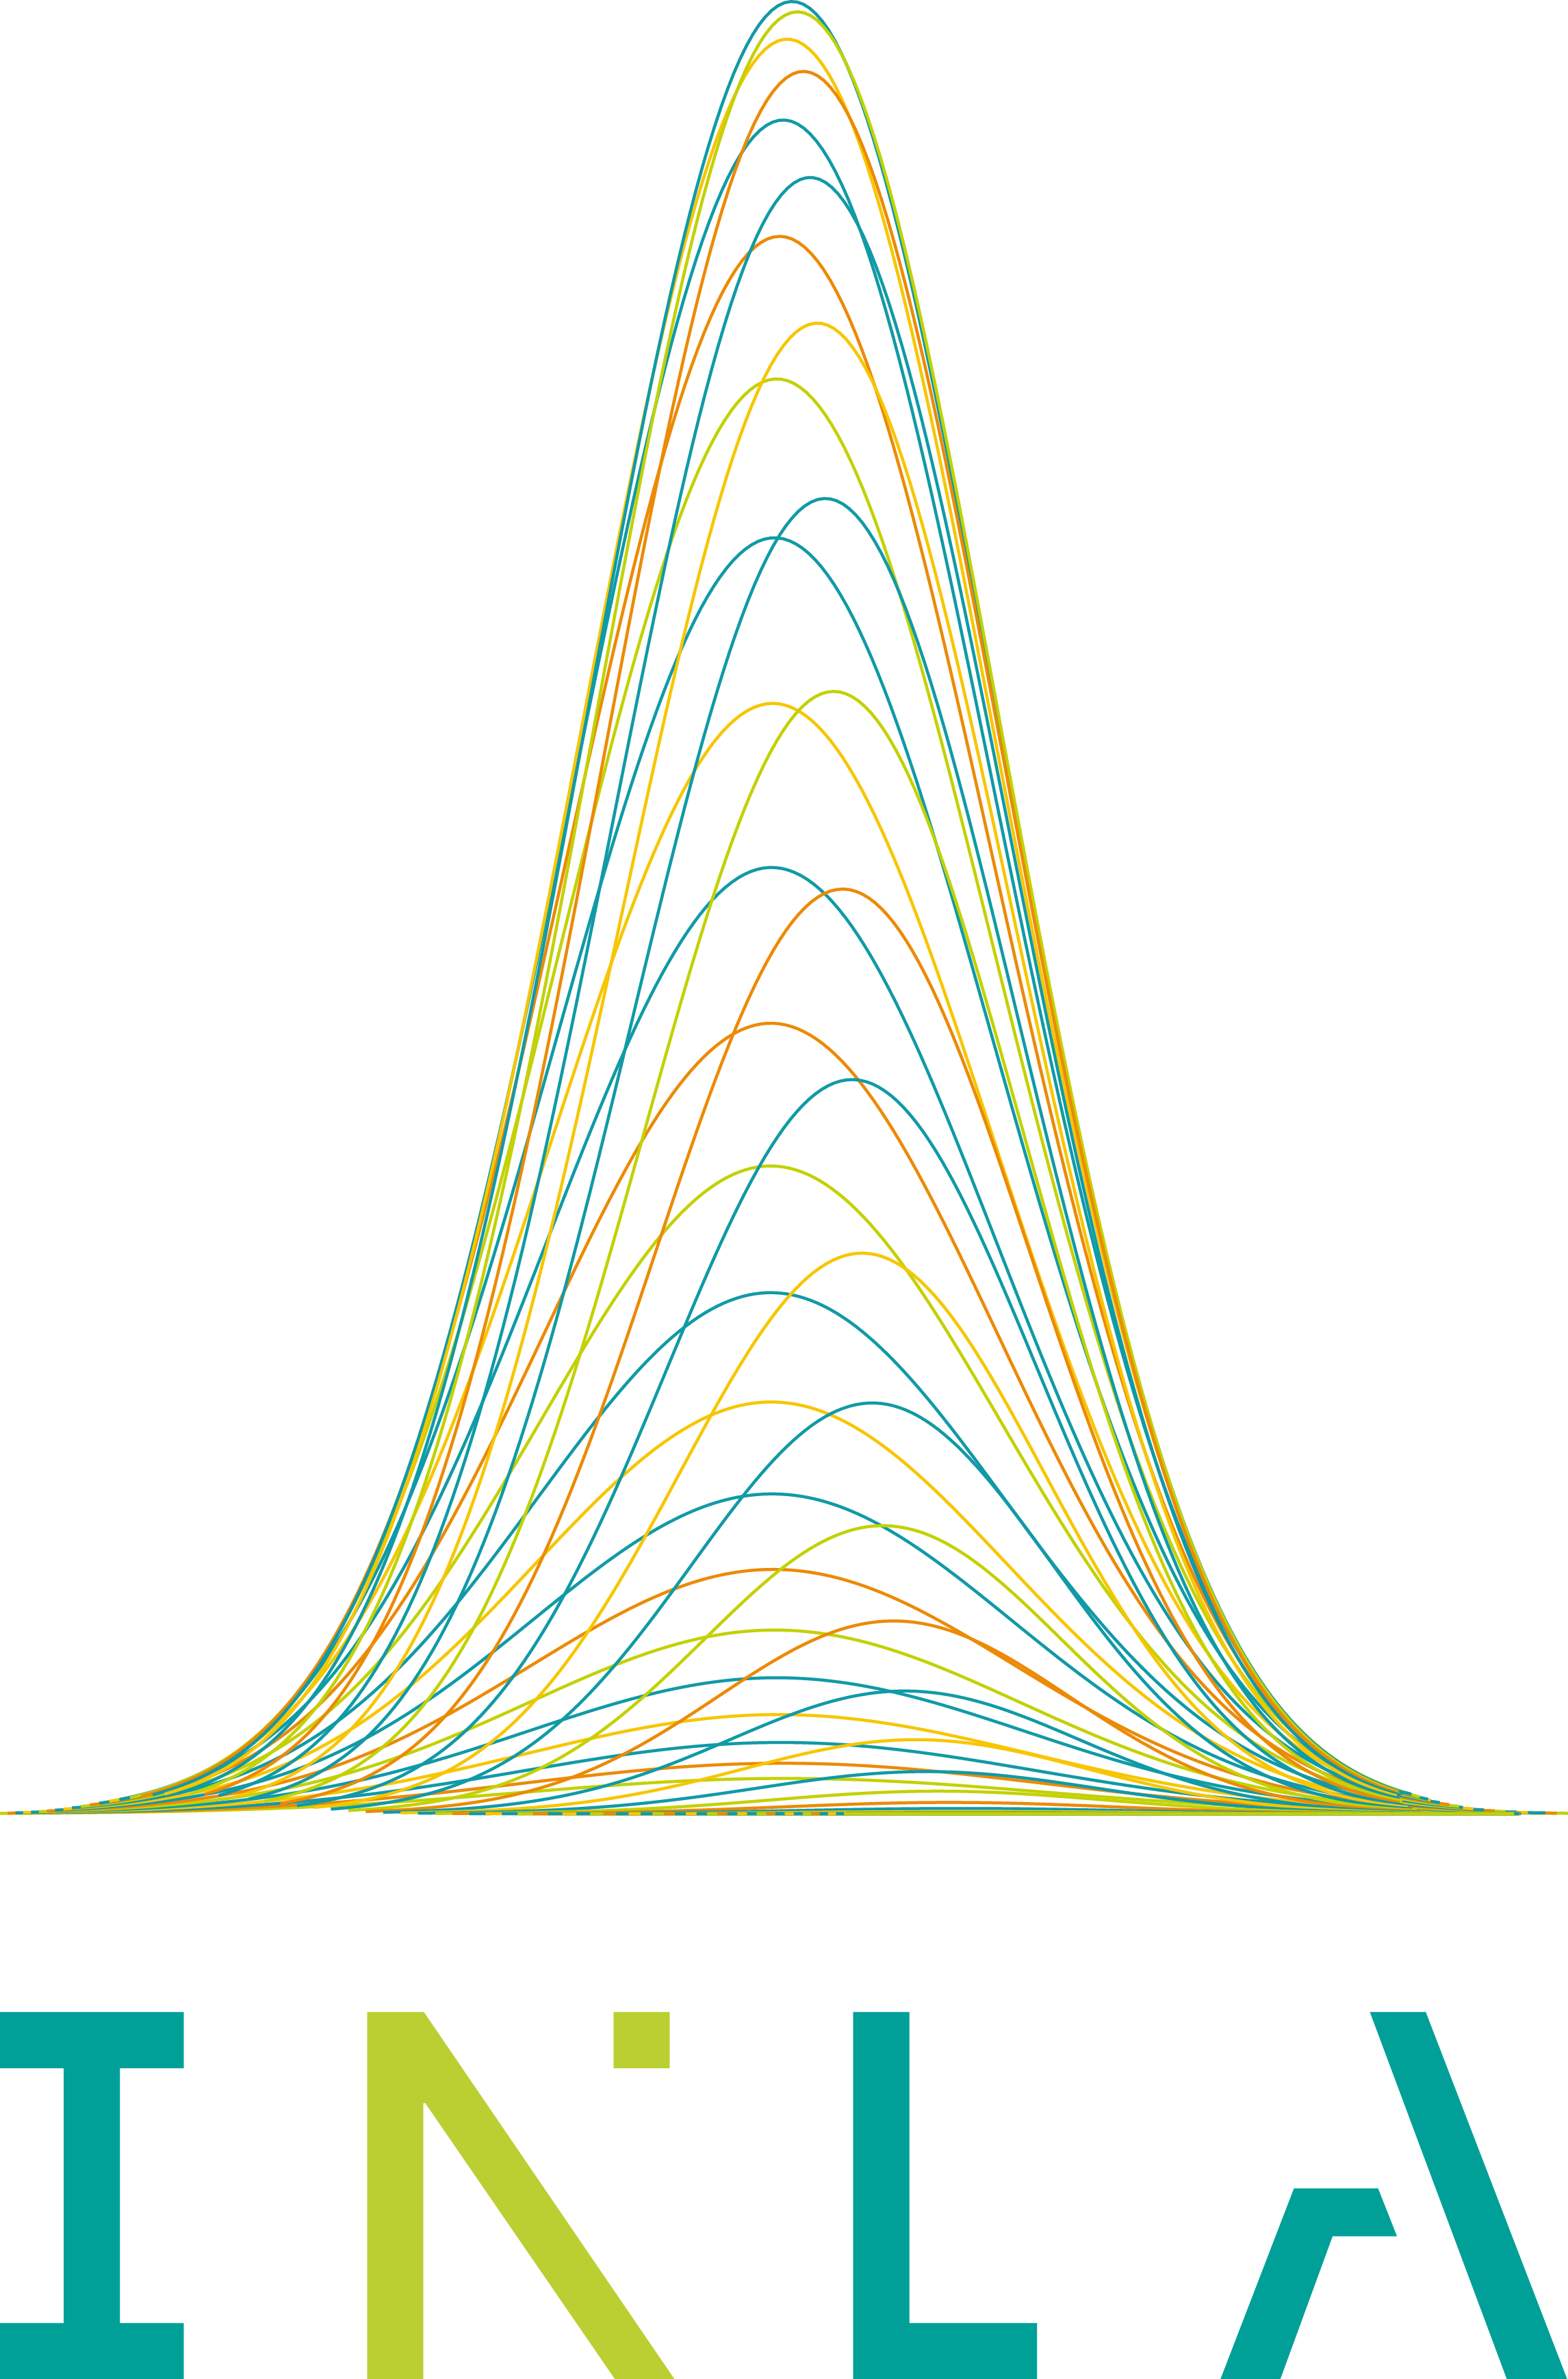
\includegraphics[scale=0.2]{data/inlalogo.png}
		\HRule{0.5pt} \\ [0.5cm]
		\Large \textbf{A Smart Numerical Gradient}
		\HRule{0.5pt} \\ [0.5cm]
		\normalsize \today \vspace*{5\baselineskip}}
	
	\date{}
	
	\author{
    \\ \\
    Bayesian Computational Statistics and Modeling Research Group\\
		King Abdullah University of Science and Technology}
	
	
	\maketitle
	\thispagestyle{empty}
	
	\newpage
	\clearpage
	\thispagestyle{empty}
	\tableofcontents
	
	\newpage
	\clearpage
	\setcounter{page}{1}

	\newpage
	
\section{Test Some Functions}

\begin{figure}[H] 
	\label{ fig7} 
	\begin{minipage}[b]{0.5\linewidth}
		\centering
		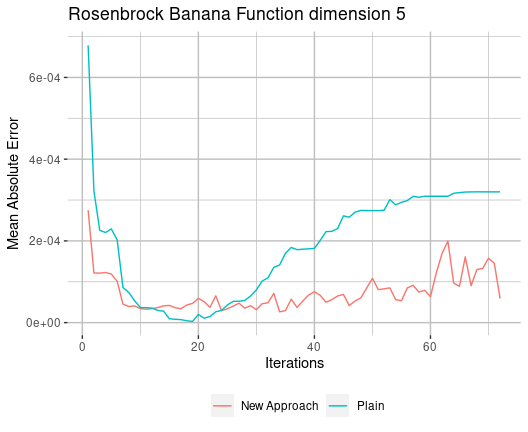
\includegraphics[scale=0.5]{plots/Rosenbrock_Banana_dim5.png} 
		\caption{MSE of Rosenbrock Function (Dim 5)} 
		\vspace{4ex}
	\end{minipage}%%
	\begin{minipage}[b]{0.5\linewidth}
		\centering
		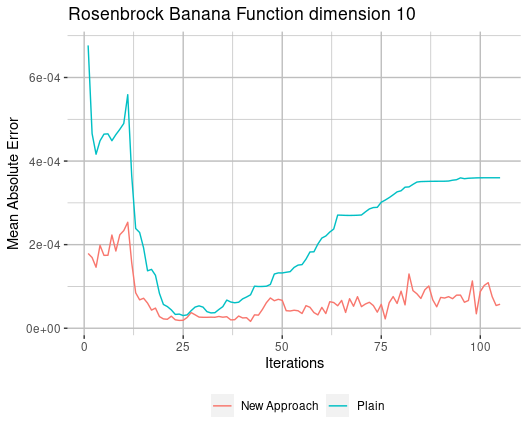
\includegraphics[scale=0.5]{plots/Rosenbrock_Banana_dim10.png} 
		\caption{Rosenbrock Function (Dim 10)} 
		\vspace{4ex}
	\end{minipage} 
	\begin{minipage}[b]{0.5\linewidth}
		\centering
		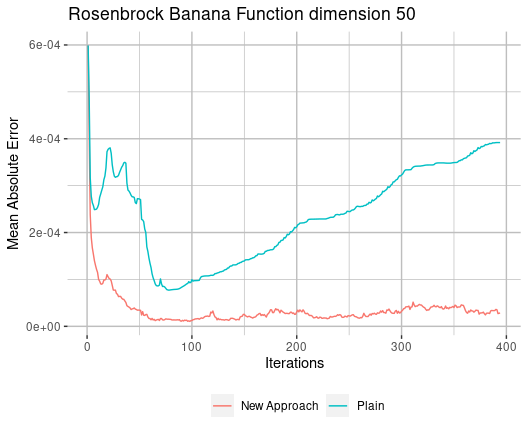
\includegraphics[scale=0.5]{plots/Rosenbrock_Banana_dim50.png} 
		\caption{Rosenbrock Function (Dim 50)} 
		\vspace{4ex}
	\end{minipage}%% 
	\begin{minipage}[b]{0.5\linewidth}
		\centering
		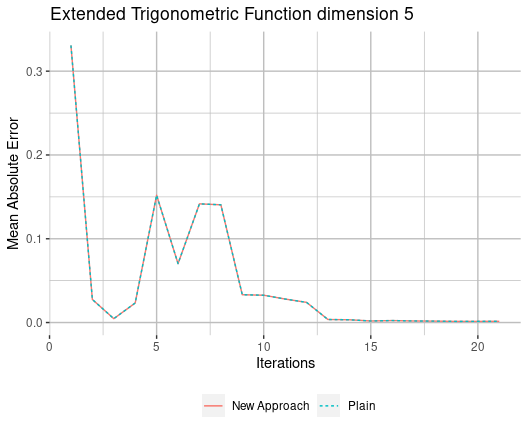
\includegraphics[scale=0.5]{plots/Extended_Trigonometric_dim5.png} 
		\caption{Ext. Trigonometric Function (Dim 5)} 
		\vspace{4ex}
	\end{minipage} 
	\begin{minipage}[b]{0.5\linewidth}
	\centering
	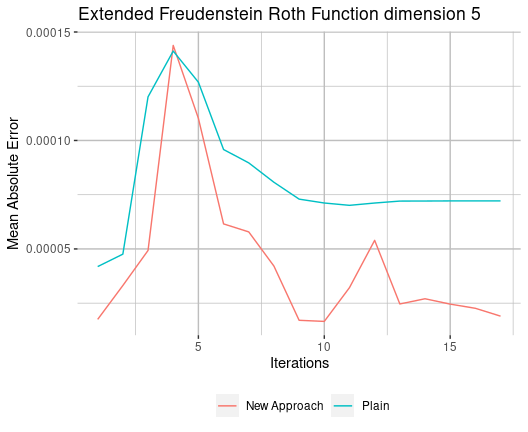
\includegraphics[scale=0.5]{plots/Extended_Freudenstein_Roth_dim5.png} 
	\caption{Ext. Freudenstein Roth Function (Dim 5)} 
	\vspace{4ex}
\end{minipage}%% 
\begin{minipage}[b]{0.5\linewidth}
	\centering
	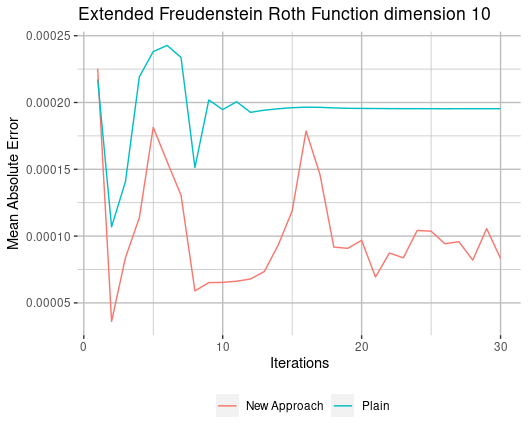
\includegraphics[scale=0.5]{plots/Extended_Freudenstein_Roth_dim10.png} 
	\caption{Ext. Freudenstein Roth Function (Dim 10)} 
	\vspace{4ex}
\end{minipage} 
\end{figure}

\begin{figure}[H] 
	\label{ fig7} 
	\begin{minipage}[b]{0.5\linewidth}
		\centering
		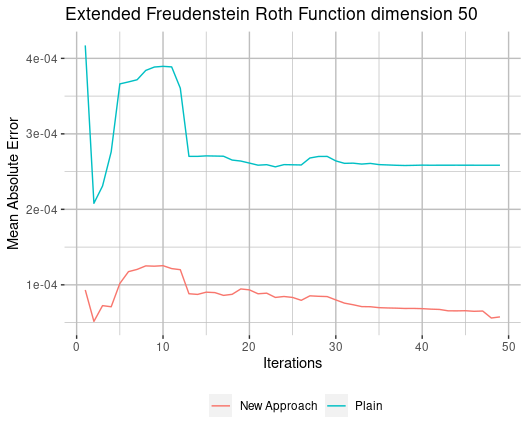
\includegraphics[scale=0.5]{plots/Extended_Freudenstein_Roth_dim50.png} 
		\caption{Ext. Freudenstein Roth Function (Dim 50)} 
		\vspace{4ex}
	\end{minipage}%%
	\begin{minipage}[b]{0.5\linewidth}
		\centering
		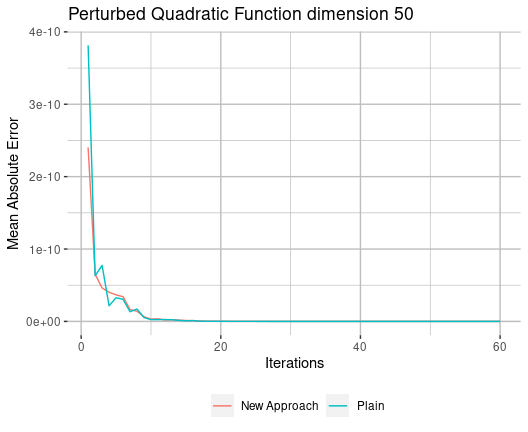
\includegraphics[scale=0.5]{plots/Perturbed_Quadratic_Function_dim50.png} 
		\caption{Perturbed Quadratic Function (Dim 50)} 
		\vspace{4ex}
	\end{minipage} 
	\begin{minipage}[b]{0.5\linewidth}
		\centering
		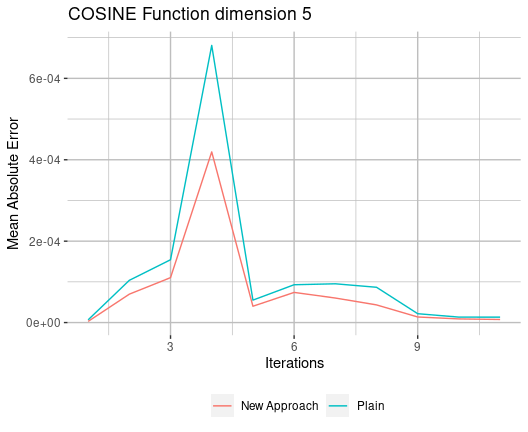
\includegraphics[scale=0.5]{plots/COSINE_dim5.png} 
		\caption{COSINE Function (Dim 50)} 
		\vspace{4ex}
	\end{minipage}%% 
	\begin{minipage}[b]{0.5\linewidth}
		\centering
		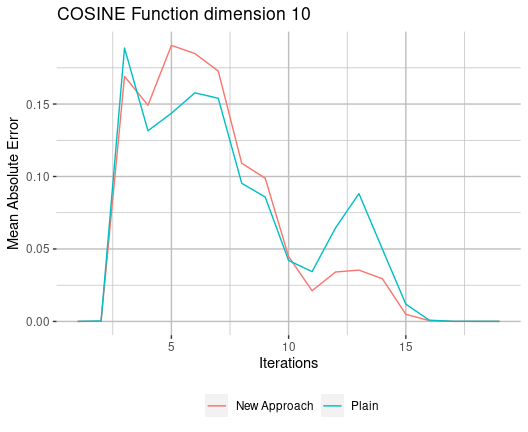
\includegraphics[scale=0.5]{plots/COSINE_dim10.png}  
		\caption{COSINE Function (Dim 10)} 
		\vspace{4ex}
	\end{minipage} 
	\begin{minipage}[b]{0.5\linewidth}
		\centering
		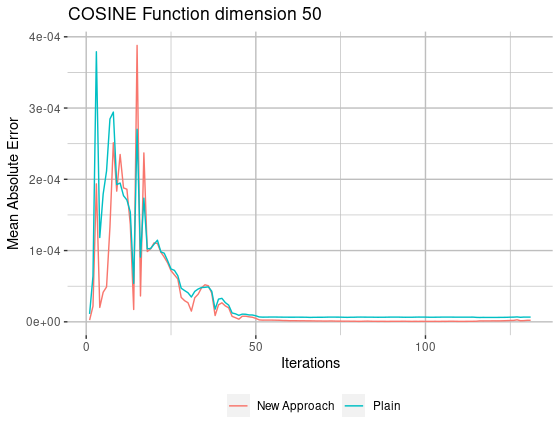
\includegraphics[scale=0.5]{plots/COSINE_dim50.png}  
		\caption{COSINE Function (Dim 50)} 
		\vspace{4ex}
	\end{minipage}%% 
	\begin{minipage}[b]{0.5\linewidth}
		\centering
		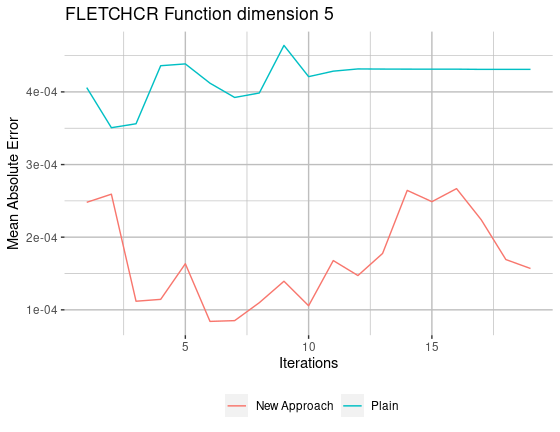
\includegraphics[scale=0.5]{plots/FLETCHCR_dim5.png} 
		\caption{FLETCHCR Function (Dim 5)} 
		\vspace{4ex}
	\end{minipage} 
\end{figure}

\begin{figure}[H] 
	\label{ fig7} 
	\begin{minipage}[b]{0.5\linewidth}
		\centering
		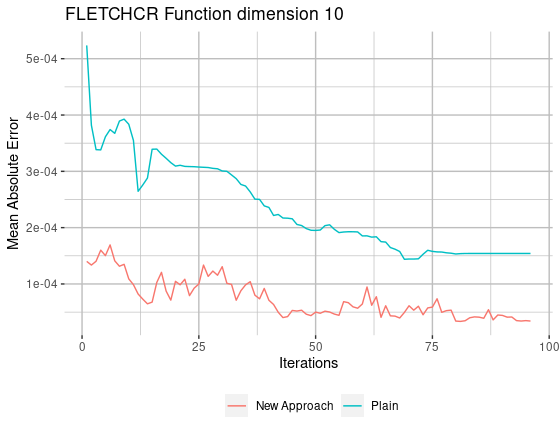
\includegraphics[scale=0.5]{plots/FLETCHCR_dim10.png} 
		\caption{FLETCHCR Function (Dim 10)} 
		\vspace{4ex}
	\end{minipage}%%
	\begin{minipage}[b]{0.5\linewidth}
		\centering
		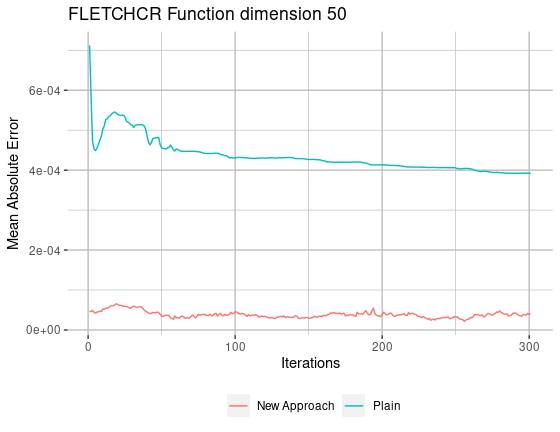
\includegraphics[scale=0.5]{plots/FLETCHCR_dim50.png} 
		\caption{FLETCHCR Function (Dim 50)} 
		\vspace{4ex}
	\end{minipage} 
	\begin{minipage}[b]{0.5\linewidth}
		\centering
		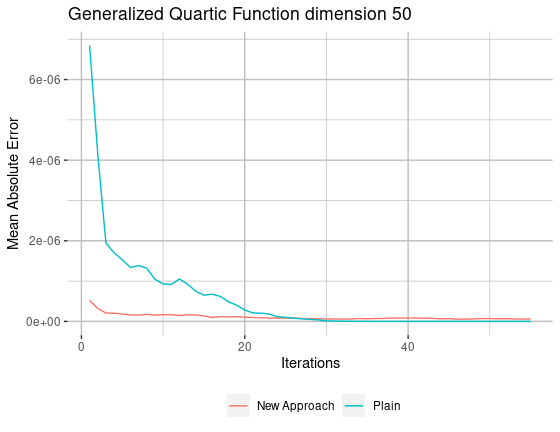
\includegraphics[scale=0.5]{plots/Generalized_Quartic_dim50.png} 
		\caption{Generalized Quartic Function (Dim 50)} 
		\vspace{4ex}
	\end{minipage}%% 
	\begin{minipage}[b]{0.5\linewidth}
		\centering
		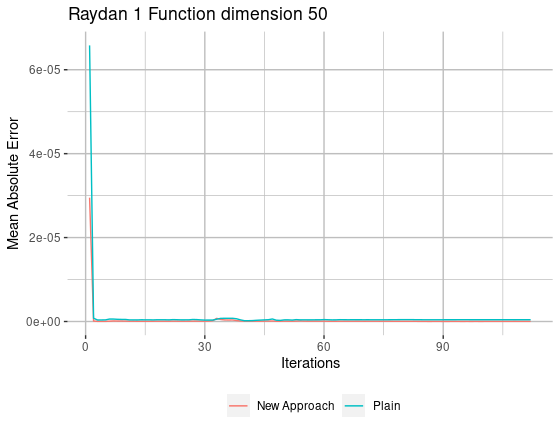
\includegraphics[scale=0.5]{plots/Raydan_1_dim50.png}  
		\caption{Raydan 1 Function (Dim 50)} 
		\vspace{4ex}
	\end{minipage} 
\end{figure}


\begin{table}[H]
	\begin{tabular}{|l|c|c|c|}
		\hline
		\multicolumn{1}{|c|}{\textbf{Function}}                            & \textbf{$x$ dimension} & \textbf{\begin{tabular}[c]{@{}c@{}}Average MSE \\ 100 iterations\\ Default Approach\end{tabular}} & \textbf{\begin{tabular}[c]{@{}c@{}}Average MSE \\ 100 iterations\\ New Approach\end{tabular}} \\ \hline
		\textbf{Rosenbrock Banana Function}                                & 5                      & 0.00026                                                                                           & 0.000104                                                                                      \\ \hline
		\textbf{Rosenbrock Banana Function}                                & 10                     & 0.000271                                                                                          & 7.8e-05                                                                                       \\ \hline
		\textbf{Rosenbrock Banana Function}                                & 50                     & 0.000292                                                                                          & 7.8e-05                                                                                       \\ \hline
		\textbf{Rosenbrock Banana Function}                                & 100                    &                                                                                                   &                                                                                               \\ \hline
		\textbf{Extended Trigonometric Function}                           & 5                      & 0.048934                                                                                          & 0.048932                                                                                      \\ \hline
		\textbf{Extended Trigonometric Function}                           & 10                     &                                                                                                   &                                                                                               \\ \hline
		\multicolumn{1}{|c|}{\textbf{Extended Freudenstein Roth Function}} & 5                      & 0.000226                                                                                          & 0.000137                                                                                      \\ \hline
		\multicolumn{1}{|c|}{\textbf{Extended Freudenstein Roth Function}} & 10                     & 0.000262                                                                                          & 0.000132                                                                                      \\ \hline
		\textbf{Extended Freudenstein Roth Function}                       & 50                     & 0.000299                                                                                          & 0.000106                                                                                      \\ \hline
		\textbf{Perturbed Quadratic Function}                              & 50                     & 0                                                                                                 & 0                                                                                             \\ \hline
		\textbf{COSINE Function}                                           & 5                      & 0.0123                                                                                            & 0.007932                                                                                      \\ \hline
		\textbf{COSINE Function}                                           & 10                     & 1.199679                                                                                          & 1.016674                                                                                      \\ \hline
		\textbf{COSINE Function}                                           & 50                     & 0.181691                                                                                          & 0.142211                                                                                      \\ \hline
		\textbf{FLETCHCR Function}                                         & 5                      & 0.000318                                                                                          & 0.000139                                                                                      \\ \hline
		\textbf{FLETCHCR Function}                                         & 10                     & 0.000327                                                                                          & 0.000104                                                                                      \\ \hline
		\textbf{FLETCHCR Function}                                         & 50                     & 0.000361                                                                                          & 4e-05                                                                                         \\ \hline
		\textbf{Generalized Quartic Function}                              & 50                     & 1e-06                                                                                             & 0                                                                                             \\ \hline
		\textbf{Raydan 1 Function}                                         & 50                     & 1e-06                                                                                             & 0                                                                                             \\ \hline
	\end{tabular}
\end{table}

\end{document}